\documentclass{article}
\usepackage{graphicx}
\usepackage[margin=1.5cm]{geometry}
\usepackage{amsmath}

\begin{document}
\twocolumn

\title{Wednesday warm-up: Forces II}
\author{Prof. Jordan C. Hanson}

\maketitle

\section{Memory Bank}

\begin{itemize}
\item Force of drag, in air or other gas: $F_D = \frac{1}{2}C \rho A v^2$.
\item In the above formula, $C$ is an empirical constant, $\rho$ is the density of the air or gas, $A$ is the area of the object, and $v$ is the object's velocity.
\item Position during uniform circular motion, with angular velocity $\omega = \Delta \theta / \Delta t$:
\begin{equation}
\vec{r}(t) = r\cos(\omega t)\hat{i} + r\sin(\omega t)\hat{j} \label{eq:1}
\end{equation}
\end{itemize}

\section{Centripetal Force}

\begin{enumerate}
\item Use Eq.\ref{eq:1} to prove the following relationships for a system in uniform circular motion.
\begin{itemize}
\item The tangent velocity:
\begin{equation}
\vec{v}(t) = -r\omega \cos(\omega t)\hat{i} +  r\omega\sin(\omega t)\hat{j}
\end{equation}
\item The centripetal acceleration:
\begin{equation}
\vec{v}(t) = -r\omega \cos(\omega t)\hat{i} +  r\omega\sin(\omega t)\hat{j}
\end{equation}
\item Magnitude of $\vec{v}$: $v = r\omega$
\item Magnitude of $\vec{a}$: $a_{\rm C} = r\omega^2$
\end{itemize} \vspace{3cm}
\item Consider the banking plane in Fig. \ref{fig:1}.  Suppose the mass of the plane is $10^4$ kg.  (a) If the lift force $\vec{L}$ has a magnitude of $1.02 \times 10^5$ N, what is the bank angle such that the plane flies level? (b) What is the centripetal force? (c) Note that the \textit{period} $T$ of circular motion is $T = 2\pi/\omega$.  If the period of the circular motion of the plane is 2 minutes, what is the radius of curvature of the path? \\ \vspace{3cm}
\item Consider the centrifuge in Fig. \ref{fig:2}.  (a) If the radius of the path of the substance in the glass vial is 10 cm, and the vial goes around the circle 600 times per minute (600 rpm), what is the centripetal acceleration? (b) Divide this result by $g$. \\ \vspace{2cm}
\end{enumerate}

\begin{figure}[hb]
\centering
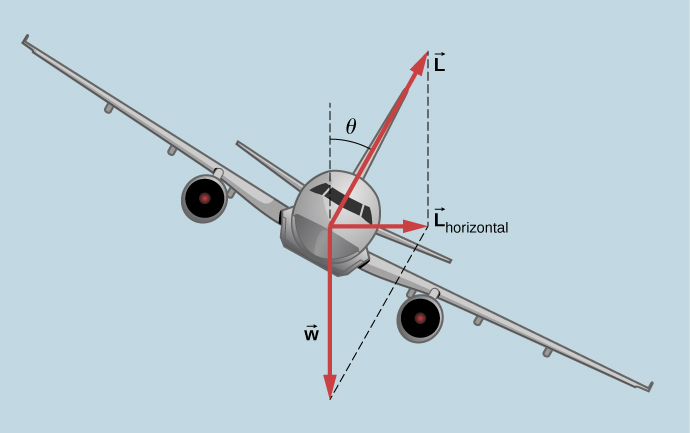
\includegraphics[width=0.35\textwidth]{figures/plane.jpeg}
\caption{\label{fig:1} A plane banks with an angle $\theta$ relative to vertical.  The force of lift is $\vec{L}$.}
\end{figure}

\begin{figure}[hb]
\centering
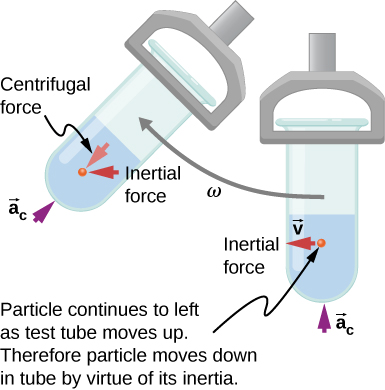
\includegraphics[width=0.35\textwidth]{figures/cent.jpeg}
\caption{\label{fig:2} A centrifuge converts centripetal acceleration into ``centrifugal force.''}
\end{figure}

\end{document}
